\documentclass{article}
\usepackage{tikz}
\usepackage{pgfplots}
\usepackage{xcolor}
\usepackage{graphicx}

\pgfplotsset{compat=1.18}

\pagecolor{red!20!black}

\begin{document}

\def\step{2}
\def\lst{0}
\def\scaleval{1.4}
\def\shoot{0}
\def\demon{1}
\def\gameover{1}
\def\score{2}


\begin{center}

\begin{tikzpicture}[scale=\scaleval]

    \pgfmathsetmacro{\W}{15}
    \pgfmathsetmacro{\H}{8}

    %\fill[red!20!black] (-0.0 * \W, -0.9 * \H) rectangle (\W + 0.0 * \W, \H + 0.9 * \H);

    \pgfmathsetmacro{\N}{9 - 2*\step}
    \pgfmathsetmacro{\cell}{\W / \N}

    \pgfmathsetmacro{\mid}{(\N - 1) / 2}

    \pgfmathsetmacro{\xA}{\mid * \cell}
    \pgfmathsetmacro{\xB}{(\mid + 1) * \cell}
    
    % make it square
    \pgfmathsetmacro{\size}{\xB - \xA}
    
    \pgfmathsetmacro{\yA}{(\H - \size)/2}
    \pgfmathsetmacro{\yB}{\yA + \size}

    \draw[thick, fill=red!15!black] (\xA,\yA) rectangle (\xB,\yB);

    % drawing wall

    \pgfmathsetmacro{\sizeRef}{\size}

    \pgfmathsetmacro{\xALast}{\xA}
    \pgfmathsetmacro{\xBLast}{\xB}
    \pgfmathsetmacro{\yALast}{\yA}
    \pgfmathsetmacro{\yBLast}{\yB}

    \foreach \i in \lst {
    
        \pgfmathsetmacro{\offset}{\size * (2^\i)}
        \pgfmathsetmacro{\yext}{\offset / 2}
    
        \ifcase\i
            \def\wallcolor{black}
        \else
            \pgfmathsetmacro{\shade}{int(2 + 15*\i)}
            \edef\wallcolor{red!\shade!black}
        \fi
    
        % LEFT
        \pgfmathsetmacro{\xAi}{\xALast - \offset}
        \fill[fill=\wallcolor, draw=black]
            (\xAi,\yALast-\yext)
            -- (\xAi,\yBLast+\yext)
            -- (\xALast,\yBLast)
            -- (\xALast,\yALast)
            -- cycle;
    
        % RIGHT
        \pgfmathsetmacro{\xBi}{\xBLast + \offset}
        \fill[fill=\wallcolor, draw=black]
            (\xBi,\yALast-\yext)
            -- (\xBi,\yBLast+\yext)
            -- (\xBLast,\yBLast)
            -- (\xBLast,\yALast)
            -- cycle;
   
        % GROUND
        \fill[fill=red!20!black, draw=black]
            (\xALast,\yALast)
            -- (\xBLast,\yALast)
            -- (\xBi,\yALast - \yext)
            -- (\xAi,\yALast - \yext)
            -- cycle;

        % CEILING
        \fill[fill=red!20!black, draw=black]
            (\xALast,\yBLast)
            -- (\xBLast,\yBLast)
            -- (\xBi,\yBLast + \yext)
            -- (\xAi,\yBLast + \yext)
            -- cycle;

        \pgfmathparse{\xALast - \offset}
        \xdef\xALast{\pgfmathresult}
        
        \pgfmathparse{\xBLast + \offset}
        \xdef\xBLast{\pgfmathresult}
        
        \pgfmathparse{\yALast - \yext}
        \xdef\yALast{\pgfmathresult}
        
        \pgfmathparse{\yBLast + \yext}
        \xdef\yBLast{\pgfmathresult}

    }

    \pgfmathsetmacro{\weaponY}{\yALast / \scaleval}
    \pgfmathsetmacro{\demonY}{\weaponY + 0.1 * \H}

    \ifnum\demon=1
    \node at ({\W/2}, {\demonY}) { 
        
\includegraphics[width=6 cm]{demon.png}
    };
    \fi

    \ifnum\shoot=0
    \node at ({\W/2}, {\weaponY}) { 
        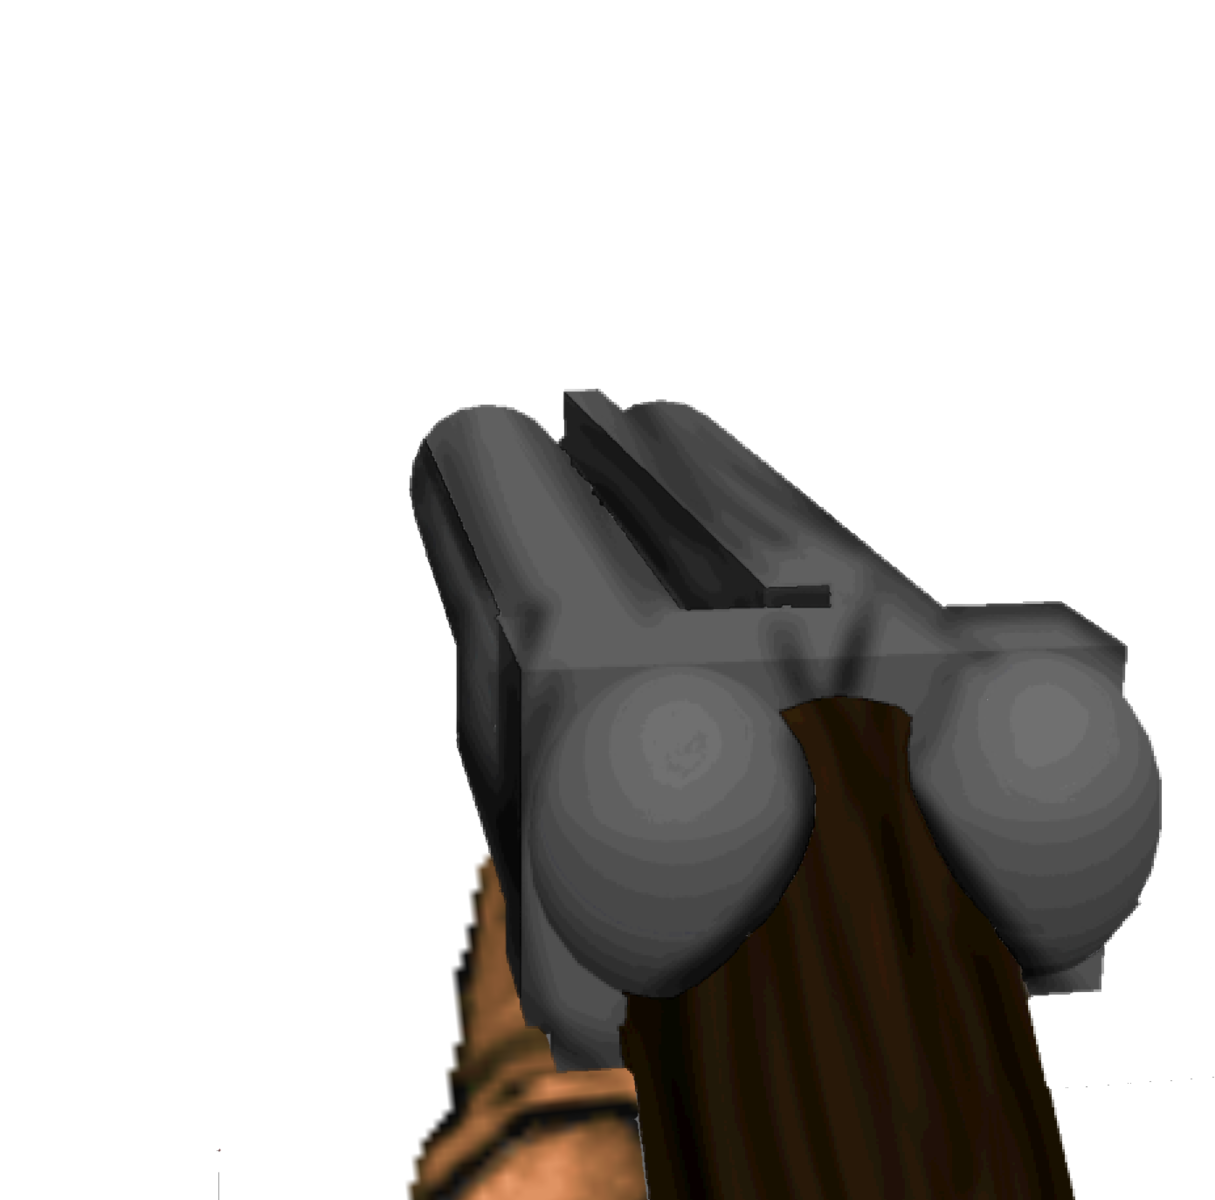
\includegraphics[width=6 cm]{weapon.png}
    };
    \else
    \node at ({\W/2}, {\weaponY}) { 
        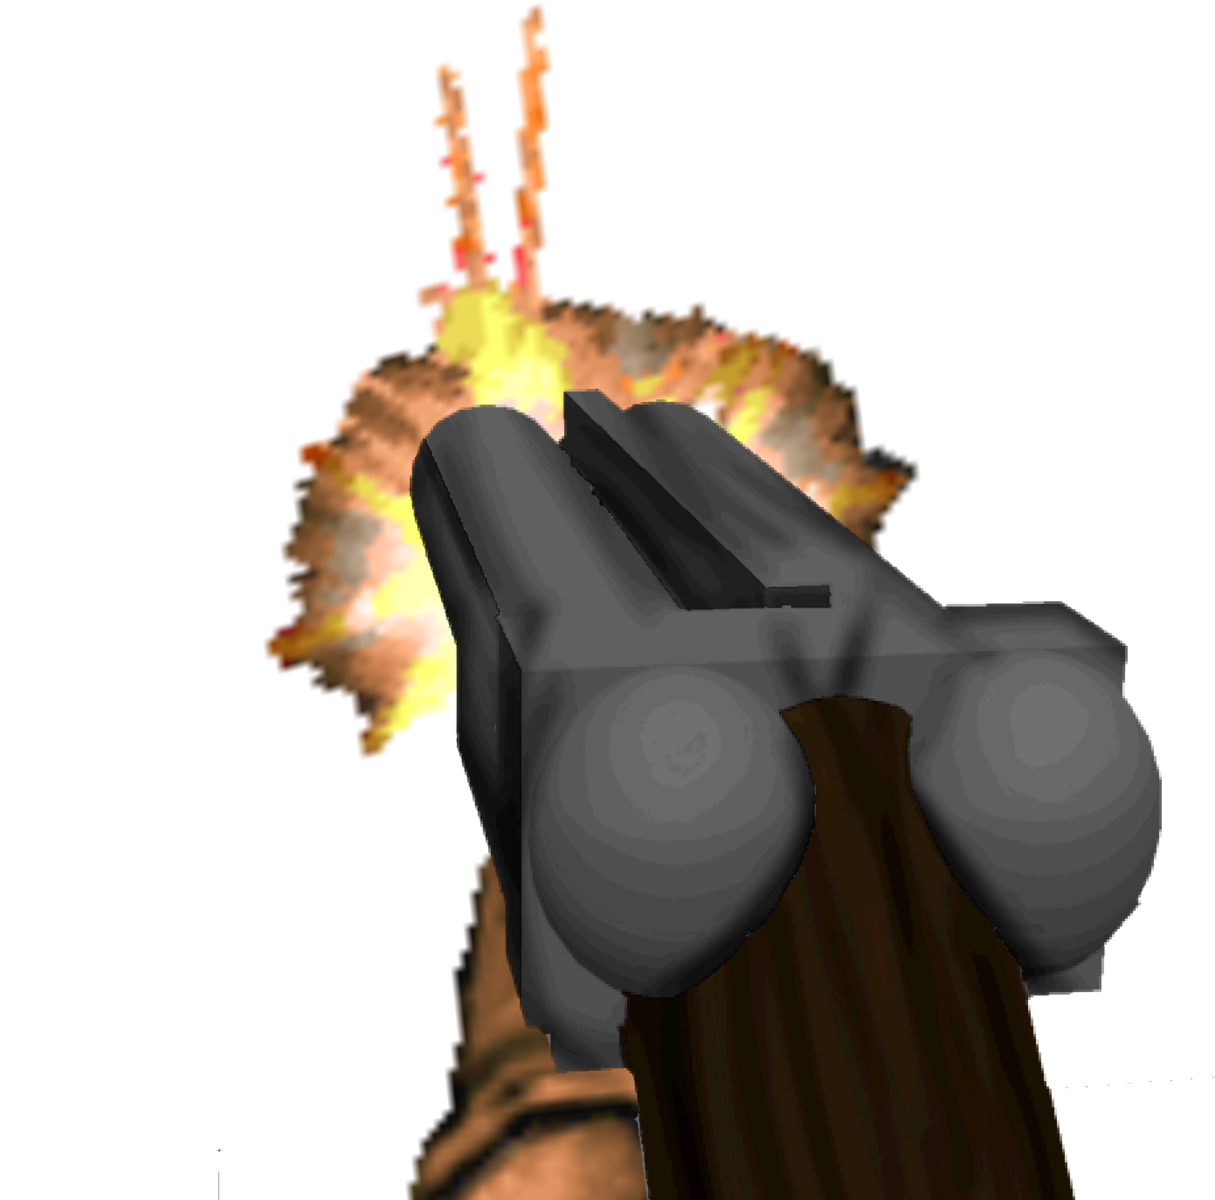
\includegraphics[width=6 cm]{weapon_shoot.png}
    };
    \fi

    \ifnum\gameover=1
    \node[white, scale=3] at ({\W/2}, {\H/2}) {GAME OVER};
    \node[red!70!black, scale=3] at ({\W/2}, {\H/2 + 1}) {SCORE: \score};
    \fi

\end{tikzpicture}
\end{center}

\end{document}






